\section{Random Walk on Networks}

The study of random walks on networks is fundamental in understanding various dynamical processes, such as diffusion, search algorithms, and transport phenomena. In this section, we formalize the mathematical framework of random walks on networks and explore their key properties, including stationary distributions, transition probabilities, and their connection to the Laplacian matrix.

Consider a network $G(N,M)$ where a particle moves randomly between the nodes at each time step, with transition probability $P_{ij}$ to go to the node $j$ starting from the node $i$. If the link between them does not exist then $P_{ij}= 0$. 
The dynamics of this system behaves as a Markov chain: it has no memory of the past states and the future state depends only on the current position.
Let $\rho_i(n)$ be the probability of finding the particle at the node $i$ at time step $n$. The discrete time evolution of the system is given by the law
\begin{equation}
    \rho_i(n+1) = \sum_j P_{ij}\rho_j(n).
\end{equation}

In order to conserve the total probability the transition probability must be a stochastic matrix, namely it must hold 
\begin{equation}
    \sum_i P_{ij}(\Delta t) = 1 .
\end{equation}

The transition probability can be identified with the adjacency matrix of the network
\begin{equation}
    P_{ij} = \frac{A_{ij}}{\sum_j A_{ij}}.
\end{equation}

If the system holds the detailed balance condition
\begin{equation}\label{detail_condition}
    \pi_{ij} \rho_j^* = \pi_{ji} \rho_i^*
\end{equation}
the system admits a unique stationary solution $\rho^*$ such that
\begin{equation}
    \sum_j P_{ij}\rho^*_j =  \rho^*_i .
\end{equation}
This can be written in matrix formalism, where $\Pi$ is the matrix of the transition probability and $\rho^*(t)$ is the stationary probability vector, as
\begin{equation}
    \Pi \rho^* = \rho^*.
\end{equation}
Tus, the stationary distribution is the eigenvector corresponding to the eigenvalue $1$ of the transition matrix.


Taking the continuum limit, we obtain the master equation \cite{Classic_random_walk}
\begin{equation}\label{master_eq}
    \dot \rho_i(t) = \sum_j \pi_{ij}\rho_j(t) - \pi_{ji}\rho_i(t) = - \sum_j L_{ij} \rho_j(t),
\end{equation}
where $\pi_{ij}$ is the transition rate, namely the transition probability per units of time, and $L_{ij} = \sum_k \pi_{kj}\delta_{ij} -\pi_{ij} $ is the Laplacian matrix.
The first term represents incoming transitions to node $i$, while the second term accounts for outgoing transitions.

The Laplacian matrix has the property that $L_{ij} < 0 $ for $i \neq j$ and also it satisfies the relation
\begin{equation}
    \sum_i L_{ij} = 0 .
\end{equation} 

The eigenvalues of the Laplacian matrix have always a not negative real part and its spectrum contains at least one zero eigenvalue, therefore it is not invertible \cite{Boccaletti}. The multiplicity of the zero eigenvalue is equal to the number of connected component of the network: in fact that if the network is not connected the Laplacian should be a block matrix,  block for each connected component, each component can be seen as an independent network with their zero eigenvalue.

The solution of master equation \eqref{master_eq} is
\begin{equation}\label{random_walk_solution}
    \rho(t) = e^{-tL}\rho(0).
\end{equation}

The master equation, in the matrix formalism, for the stationary distribution reduces to 
\begin{equation}\label{stationary_distribution}
    \dot \rho^*(t) = -L \rho^*(t) = 0 . 
\end{equation}
Thus, the stationary distribution is the eigenvector with eigenvalue $0$ of the Laplacian matrix. 
%The other eigenvalues are connected to the Ljapunov exponent and to the time that the occurs to converge to $\rho^*$.

We can prove that
\begin{equation}
    \sum_i \dot\rho_i(t) = - \sum_i \sum_j L_{ij} \rho_j(t) = - \sum_j \left(\sum_i L_{ij}\right) \rho_j(t) = 0 .
\end{equation}
This implies a first integral of motion 
\begin{equation}
    \sum_i \rho_i(t) = \sum_i \rho_i(0) .
\end{equation}

%%add the part with the measure of the eigenvalue, i.e. sum_{\lamda \neq 0} v_\lambda(t) = 0

Let us now assume the network satisfies the detailed balance condition \eqref{detail_condition}, then there exists a hyperplane $\Sigma_0$ that is orthogonal to the stationary distribution and this subspace is invariant under the dynamics. Let be $w \in \Sigma_0$, this subspace is identify by the relation
\begin{equation}
    \sum_i w_i = 0 
\end{equation}
As a matter of fact, let $w(t) \in \Sigma_0$ then 
\begin{equation}
    \sum_i w_i(t+1) = \sum_{ij} \pi_{ij} w_j(t) = \sum_j \underbrace{\left(\sum_i \pi_{ij}\right)}_{1} w_j = \sum_j w_j(t) = 0.
\end{equation}

Therefore, any probability vector can be decomposed as a direct sum of the stationary state and a vector $w(t) \in \Sigma_0$ 
\begin{equation}
    \rho(t) = \rho^* + w(t).
\end{equation}

Furthermore, if the detailed balance condition holds \eqref{detail_condition}, the stationary distribution  is \cite{Classic_random_walk}
\begin{equation}
    \rho^* = \frac{1}{N} \left(1,1,\cdots,1,1\right).
\end{equation} 

The uncertainty in the particle's location can be captured by the Shannon entropy
\begin{equation}
    S = -\sum_i p_i\ln p_i.
\end{equation}
It is a bounded function $0\geq S \geq \ln N$.
It can been shown that the stationary distribution maximizes the Shannon entropy $S = \ln N$.
    
\begin{comment}
    In figure \ref{fig:node_0} is shown only the probability to be in the initial node as a function of time starting  from a Dirac delta distribution for different types of networks\footnote{The python scripts can be found in the GitHub page of the author at the link: \url{https://github.com/ShqemzaMatteo/Master_thesis}}: a ring graph, an Erd\H{o}s-Rényi (E-R) random graph\cite{erdos-renyi1960}, a Barab\'asi-Albert (B-A) scale-free graph\cite{Barabasi_Albert_1999}, and a Watts-Strogatz (W-S) small-sworld graph\cite{Watts-Strogatz_1998}. All the algorithm are explained in the Appendix \Ref{Appendix_A}. 

    \begin{figure}[ht!]
        \centering
        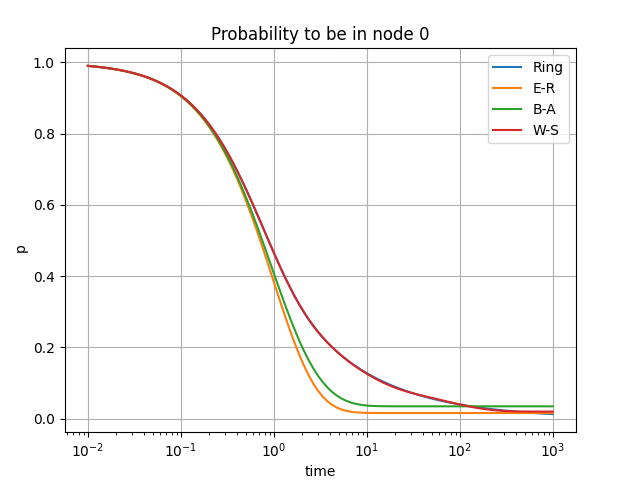
\includegraphics[width=0.65\linewidth]{image/random_graph_node_0.png}
        \caption{Plot of the probability $p$ to be in the node 0 starting from a Dirac delta distribution or the same node as a function of time for different network types of $50$ nodes: a ring graph (blue), a Erd\H{o}s-Rényi (E-R) random graph with connectivity probability $0.7$ (orange), a Barab\'asi-Albert (B-A) scale-free graph with parameter $m=3$ (green), and a Watts-Strogatz (W-S) small world graph with parameter $K=3$ and rewire probability 0.2 (red).}
        \label{fig:node_0}
    \end{figure}
\end{comment}